\documentclass[]{article}
\usepackage{lmodern}
\usepackage{amssymb,amsmath}
\usepackage{ifxetex,ifluatex}
\usepackage{fixltx2e} % provides \textsubscript
\ifnum 0\ifxetex 1\fi\ifluatex 1\fi=0 % if pdftex
  \usepackage[T1]{fontenc}
  \usepackage[utf8]{inputenc}
\else % if luatex or xelatex
  \ifxetex
    \usepackage{mathspec}
  \else
    \usepackage{fontspec}
  \fi
  \defaultfontfeatures{Ligatures=TeX,Scale=MatchLowercase}
\fi
% use upquote if available, for straight quotes in verbatim environments
\IfFileExists{upquote.sty}{\usepackage{upquote}}{}
% use microtype if available
\IfFileExists{microtype.sty}{%
\usepackage{microtype}
\UseMicrotypeSet[protrusion]{basicmath} % disable protrusion for tt fonts
}{}
\usepackage[margin=1in]{geometry}
\usepackage{hyperref}
\hypersetup{unicode=true,
            pdftitle={Compulsory exercise 2: Group XX},
            pdfauthor={NN1, NN2 and NN3},
            pdfborder={0 0 0},
            breaklinks=true}
\urlstyle{same}  % don't use monospace font for urls
\usepackage{color}
\usepackage{fancyvrb}
\newcommand{\VerbBar}{|}
\newcommand{\VERB}{\Verb[commandchars=\\\{\}]}
\DefineVerbatimEnvironment{Highlighting}{Verbatim}{commandchars=\\\{\}}
% Add ',fontsize=\small' for more characters per line
\usepackage{framed}
\definecolor{shadecolor}{RGB}{248,248,248}
\newenvironment{Shaded}{\begin{snugshade}}{\end{snugshade}}
\newcommand{\KeywordTok}[1]{\textcolor[rgb]{0.13,0.29,0.53}{\textbf{#1}}}
\newcommand{\DataTypeTok}[1]{\textcolor[rgb]{0.13,0.29,0.53}{#1}}
\newcommand{\DecValTok}[1]{\textcolor[rgb]{0.00,0.00,0.81}{#1}}
\newcommand{\BaseNTok}[1]{\textcolor[rgb]{0.00,0.00,0.81}{#1}}
\newcommand{\FloatTok}[1]{\textcolor[rgb]{0.00,0.00,0.81}{#1}}
\newcommand{\ConstantTok}[1]{\textcolor[rgb]{0.00,0.00,0.00}{#1}}
\newcommand{\CharTok}[1]{\textcolor[rgb]{0.31,0.60,0.02}{#1}}
\newcommand{\SpecialCharTok}[1]{\textcolor[rgb]{0.00,0.00,0.00}{#1}}
\newcommand{\StringTok}[1]{\textcolor[rgb]{0.31,0.60,0.02}{#1}}
\newcommand{\VerbatimStringTok}[1]{\textcolor[rgb]{0.31,0.60,0.02}{#1}}
\newcommand{\SpecialStringTok}[1]{\textcolor[rgb]{0.31,0.60,0.02}{#1}}
\newcommand{\ImportTok}[1]{#1}
\newcommand{\CommentTok}[1]{\textcolor[rgb]{0.56,0.35,0.01}{\textit{#1}}}
\newcommand{\DocumentationTok}[1]{\textcolor[rgb]{0.56,0.35,0.01}{\textbf{\textit{#1}}}}
\newcommand{\AnnotationTok}[1]{\textcolor[rgb]{0.56,0.35,0.01}{\textbf{\textit{#1}}}}
\newcommand{\CommentVarTok}[1]{\textcolor[rgb]{0.56,0.35,0.01}{\textbf{\textit{#1}}}}
\newcommand{\OtherTok}[1]{\textcolor[rgb]{0.56,0.35,0.01}{#1}}
\newcommand{\FunctionTok}[1]{\textcolor[rgb]{0.00,0.00,0.00}{#1}}
\newcommand{\VariableTok}[1]{\textcolor[rgb]{0.00,0.00,0.00}{#1}}
\newcommand{\ControlFlowTok}[1]{\textcolor[rgb]{0.13,0.29,0.53}{\textbf{#1}}}
\newcommand{\OperatorTok}[1]{\textcolor[rgb]{0.81,0.36,0.00}{\textbf{#1}}}
\newcommand{\BuiltInTok}[1]{#1}
\newcommand{\ExtensionTok}[1]{#1}
\newcommand{\PreprocessorTok}[1]{\textcolor[rgb]{0.56,0.35,0.01}{\textit{#1}}}
\newcommand{\AttributeTok}[1]{\textcolor[rgb]{0.77,0.63,0.00}{#1}}
\newcommand{\RegionMarkerTok}[1]{#1}
\newcommand{\InformationTok}[1]{\textcolor[rgb]{0.56,0.35,0.01}{\textbf{\textit{#1}}}}
\newcommand{\WarningTok}[1]{\textcolor[rgb]{0.56,0.35,0.01}{\textbf{\textit{#1}}}}
\newcommand{\AlertTok}[1]{\textcolor[rgb]{0.94,0.16,0.16}{#1}}
\newcommand{\ErrorTok}[1]{\textcolor[rgb]{0.64,0.00,0.00}{\textbf{#1}}}
\newcommand{\NormalTok}[1]{#1}
\usepackage{graphicx,grffile}
\makeatletter
\def\maxwidth{\ifdim\Gin@nat@width>\linewidth\linewidth\else\Gin@nat@width\fi}
\def\maxheight{\ifdim\Gin@nat@height>\textheight\textheight\else\Gin@nat@height\fi}
\makeatother
% Scale images if necessary, so that they will not overflow the page
% margins by default, and it is still possible to overwrite the defaults
% using explicit options in \includegraphics[width, height, ...]{}
\setkeys{Gin}{width=\maxwidth,height=\maxheight,keepaspectratio}
\IfFileExists{parskip.sty}{%
\usepackage{parskip}
}{% else
\setlength{\parindent}{0pt}
\setlength{\parskip}{6pt plus 2pt minus 1pt}
}
\setlength{\emergencystretch}{3em}  % prevent overfull lines
\providecommand{\tightlist}{%
  \setlength{\itemsep}{0pt}\setlength{\parskip}{0pt}}
\setcounter{secnumdepth}{0}
% Redefines (sub)paragraphs to behave more like sections
\ifx\paragraph\undefined\else
\let\oldparagraph\paragraph
\renewcommand{\paragraph}[1]{\oldparagraph{#1}\mbox{}}
\fi
\ifx\subparagraph\undefined\else
\let\oldsubparagraph\subparagraph
\renewcommand{\subparagraph}[1]{\oldsubparagraph{#1}\mbox{}}
\fi

%%% Use protect on footnotes to avoid problems with footnotes in titles
\let\rmarkdownfootnote\footnote%
\def\footnote{\protect\rmarkdownfootnote}

%%% Change title format to be more compact
\usepackage{titling}

% Create subtitle command for use in maketitle
\newcommand{\subtitle}[1]{
  \posttitle{
    \begin{center}\large#1\end{center}
    }
}

\setlength{\droptitle}{-2em}
  \title{Compulsory exercise 2: Group XX}
  \pretitle{\vspace{\droptitle}\centering\huge}
  \posttitle{\par}
\subtitle{TMA4268 Statistical Learning V2018}
  \author{NN1, NN2 and NN3}
  \preauthor{\centering\large\emph}
  \postauthor{\par}
  \predate{\centering\large\emph}
  \postdate{\par}
  \date{12 mars, 2018}


\begin{document}
\maketitle

\subsection{1a)}\label{a}

\begin{itemize}
\tightlist
\item
  Q1: We have \(d\) possible predictors. First of all, we can chose how
  many of these predictors we want to use. We have the choice to use
  \(k=0,1,2,\dots,d\) predictors in our model. If we use \(k=0\)
  predictors, we don't really have a linear regression model, instead we
  will get a model that predicts new samples as the average of all
  previous samples. Even though this is not a linear regression model,
  we want to investigate whether this gives a better result than using a
  linear regression model would. That would imply that there is no
  linear connection between the data from our sample. Let us now focus
  on the choices of \(k\) that results in linear regression models. If
  we choose to use \(k=1\) predictor, we again have a choice in which of
  the \(d\) possible predictors we want to use. Obviuosly there are
  \(d\) possible choices for \(k=1\), but if we want to be more
  systematic we can say that we choose \(k\) different predictors from
  \(d\) possible ones, and we can not choose the same twice. Hence, the
  number of possible combinations using \(k\) predictors is given by the
  standard nCr-formula \(\binom{d}{k}\). Now we have our \(d\) different
  choices of \(k\), which all gives different linear regression models.
  In total, the number of models is
  \[\binom{d}{1}+\binom{d}{2}+\dots+\binom{d}{d}.\]. The binomial
  theorem states that \[(1+x)^n=\sum_{k=0}^n \binom{n}{k} x^k.\]. By
  setting \(x=1\), we see that the number of different linear regression
  models is given by \[\sum_{k=1}^d \binom{d}{k}=2^d -1.\]
\item
  Q2: The following algorithm illustrates how the best subset method
  finds the best model amongst the \(2^d-1\) possible ones: Denote first
  by \(\mathcal{M}_0\) the model using no predictors. This model simply
  predicts the sample mean for new observations. Next, for
  \(k=1,2,\dots,d\), fit all \(\binom{d}{k}\) models, by solving the
  equation
  \(\hat{\boldsymbol \beta} =(\boldsymbol X^T \boldsymbol X)^{-1} \boldsymbol X^T \boldsymbol Y\),
  where \(\boldsymbol{X}\) and \(\boldsymbol{Y}\) only contains the
  predictors for one specific model. Calculate the RSS, and choose the
  model with the lowest RSS amongst the \(\binom{d}{k}\) models, to be
  considered later. Now after the for-loop, we have \(d+1\) possible
  models to consider. Calculate
  \(BIC=\frac{1}{n}(RSS+log(d)k\hat \sigma^2)\) for each, and choose the
  model with the lowest \(BIC\). This is the best model by the best
  subset method, using \(BIC\)-criterion. \(R^2\) is given by
  \(1-RSS/TSS\). In this expression, we do not care how many predictors
  are being used. This is a problem, because training error is a poor
  estimate for test error, since it may cause overfitting. A possible
  solution to this is to add penalties, depending on how many predictors
  we use. If we were to use \(R^2\) instead of \(BIC\) to choose the
  best model, our best model would surely contain all \(d\) predictors
  since over-fitting would make our model fit the training data better.
  This is unwanted as we would rather have a model that best fit test
  data, which \(BIC\) better simulates.
  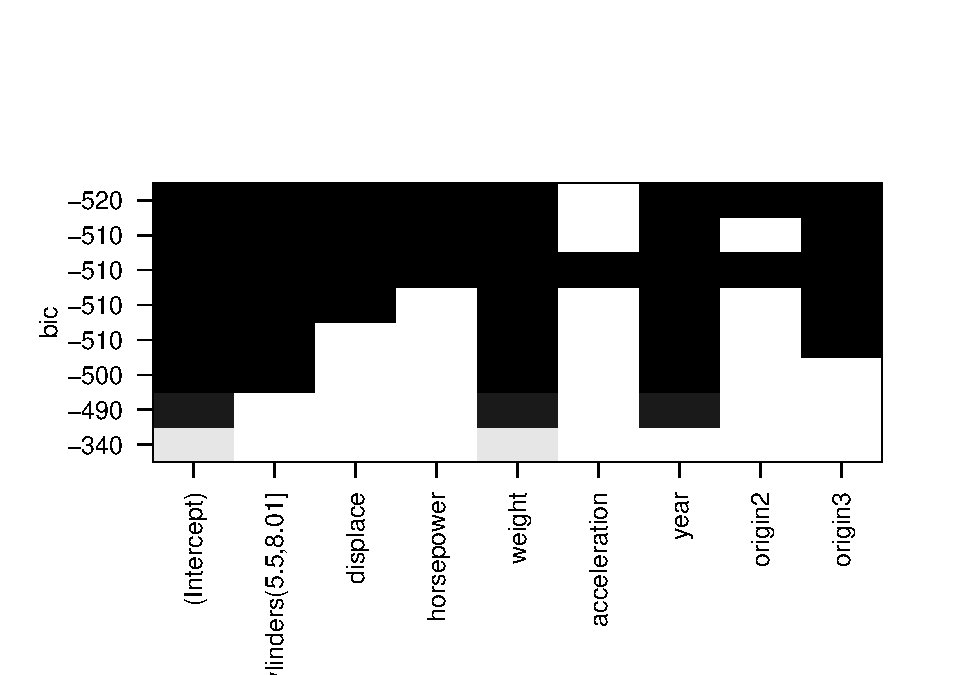
\includegraphics{1_files/figure-latex/unnamed-chunk-1-1.pdf}
\end{itemize}

\subsection{1b)}\label{b}

\begin{itemize}
\tightlist
\item
  Q3: As explained in Q2, \(RSS\) is calculated for all models, and for
  each model complexity, we choose the model with the lowest \(RSS\) as
  our best model. The \texttt{regsubsets}-function in R performs the
  actual calculations, and in the summary we can see which predictors
  corresponds to the lowest \(RSS\) for each model complexity. We see
  from this summary, which is printed in the task, that the best model
  with two predictors use the ``weight'' and ``year'' columns.
\item
  Q4: Now assuming we have the best model for each model complexity, we
  still want to choose which model complexity to use. As discussed in
  Q2, we would have the smallest \(RSS\) for the highest possible model
  complexity in the training set, but since we want to avoid
  overfitting, we add penalties to more complex models. Therefore, for
  each model complexity, we add the penalties according to the
  \(BIC\)-criterion, and then choose the model with the lowest value as
  our best method. The \(regsubsets\)-function in R also does the
  calculations for the penalties, using \(BIC\)-criterion in addition to
  other penalty-adding methods. Thus we can from the
  \texttt{regsubsets}-function also retrieve the \(BIC\)-values for each
  model complexity, and choose the lowest one as our model. The figure
  above, which is the result of plotting the \texttt{regsubsets}-data
  also contains the necessary information for choosing the best model.
  On the \(y\) scale, we see \(BIC\)-values for the models of different
  complexity, and on the \(x\)-scale we see which predictors are
  contained in the best model of this complexity, as a black box. We
  choose the model with the lowest \(BIC\)-value, which we see has
  \(BIC\sim -520\), and contains seven predictors, all but acceleration.
  Hence, this is our best model according to the best subset method
  using \(BIC\)-criterion on the training data. From the prints in the
  task we see th more exact \(BIC=-516.9417\), which was rounded off to
  -520. The following R-code fits this model to the training data, by
  using the \texttt{lm}-function. The summary output gives us
  information about how well the model fit. We see that all of the
  \(t\)-values are fairly high, and the \(p\)-values for all but one are
  within the 0.001-significance level, while the last one is within the
  0.01 significance level. We can therefore with a very high certainty
  throw away the zero hypothesis without making a mistake. We also see
  R-squared-values relatively close to 1, which indicates a good model
  fit. Also we have \(RSS=RSE^2(n-k-1)\), so that
  \[MSE=\frac{RSS}{n}=\frac{RSE^2(n-k-1)}{n}=\frac{3.233^2\cdot 305}{313}=10.185.\]
  We have also performed an Anderson-Darling test for Normality. The
  \(p\)-value for this test is \(9.241\cdot 10^-6\), which is very
  small, and indicates that our data does not have normal distributed
  errors. ???
\end{itemize}

\begin{Shaded}
\begin{Highlighting}[]
\KeywordTok{library}\NormalTok{(nortest)}
\NormalTok{trainLm=}\KeywordTok{lm}\NormalTok{(mpg}\OperatorTok{~}\NormalTok{. }\OperatorTok{-}\NormalTok{acceleration, }\DataTypeTok{data=}\NormalTok{ourAutoTrain)}
\KeywordTok{summary}\NormalTok{(trainLm)}
\KeywordTok{ad.test}\NormalTok{(}\KeywordTok{rstudent}\NormalTok{(trainLm))}
\NormalTok{yhat=}\KeywordTok{predict}\NormalTok{(trainLm,ourAutoTest)}
\KeywordTok{mean}\NormalTok{((ourAutoTest}\OperatorTok{$}\NormalTok{mpg}\OperatorTok{-}\NormalTok{yhat)}\OperatorTok{^}\DecValTok{2}\NormalTok{)}
\end{Highlighting}
\end{Shaded}

\begin{verbatim}
## 
## Call:
## lm(formula = mpg ~ . - acceleration, data = ourAutoTrain)
## 
## Residuals:
##     Min      1Q  Median      3Q     Max 
## -8.7254 -2.0561 -0.3412  1.7122 12.9550 
## 
## Coefficients:
##                       Estimate Std. Error t value Pr(>|t|)    
## (Intercept)         -1.941e+01  4.589e+00  -4.230 3.09e-05 ***
## cylinders(5.5,8.01] -3.533e+00  7.469e-01  -4.730 3.43e-06 ***
## displace             3.279e-02  6.749e-03   4.858 1.90e-06 ***
## horsepower          -4.883e-02  1.184e-02  -4.124 4.80e-05 ***
## weight              -5.824e-03  6.185e-04  -9.415  < 2e-16 ***
## year                 7.849e-01  5.699e-02  13.771  < 2e-16 ***
## origin2              1.794e+00  6.204e-01   2.892  0.00411 ** 
## origin3              2.906e+00  5.943e-01   4.891 1.63e-06 ***
## ---
## Signif. codes:  0 '***' 0.001 '**' 0.01 '*' 0.05 '.' 0.1 ' ' 1
## 
## Residual standard error: 3.233 on 305 degrees of freedom
## Multiple R-squared:  0.8344, Adjusted R-squared:  0.8306 
## F-statistic: 219.6 on 7 and 305 DF,  p-value: < 2.2e-16
## 
## 
##  Anderson-Darling normality test
## 
## data:  rstudent(trainLm)
## A = 2.2684, p-value = 9.241e-06
## 
## [1] 8.931018
\end{verbatim}

\begin{itemize}
\tightlist
\item
  Q5: The code above also predicts new values for the test set, and
  calculates the test-\(MSE\). Here, we got \(MSE=8.931\), which
  actually is smaller than the training \(MSE\), indicating that we
  indeed have managed to avoid overfitting, and made a model which
  predicts new values pretty well.
\end{itemize}

\subsection{1c)}\label{c}

\begin{itemize}
\tightlist
\item
  Q6. K-fold cross-validation involves dividing the data into \(k\)
  folds, \(C_1, C_2, \dots, C_k\). We then want to divide the data into
  a training and test set, and we choose one of the \(k\) parts as the
  test set, while we let the rest be training data. After fitting the
  model, we calculate \(MSE\) for the specific test folder, as
  \[MSE_j=\frac{a}{n_k}\sum_{i \in C_j}(y_i-\hat y_i)^2\]
\item
  Q7. Why may \(k\)-fold cross-validation be preferred to leave-one-out
  cross-validation?
\end{itemize}

\subsection{1d}\label{d}

\begin{itemize}
\tightlist
\item
  Q8. The R-code for performing 10-fold cross validation is below.
\end{itemize}

\begin{Shaded}
\begin{Highlighting}[]
\KeywordTok{library}\NormalTok{(caret)}
\KeywordTok{library}\NormalTok{(leaps)}
\NormalTok{predict.regsubsets=}\ControlFlowTok{function}\NormalTok{(object,newdata,id)\{}
\NormalTok{  form=}\KeywordTok{as.formula}\NormalTok{(object}\OperatorTok{$}\NormalTok{call[[}\DecValTok{2}\NormalTok{]])}
\NormalTok{  mat=}\KeywordTok{model.matrix}\NormalTok{(form,newdata)}
\NormalTok{  coefi=}\KeywordTok{coef}\NormalTok{(object,}\DataTypeTok{id=}\NormalTok{id)}
\NormalTok{  xvars=}\KeywordTok{names}\NormalTok{(coefi)}
\NormalTok{  mat[,xvars]}\OperatorTok\NormalTok{coefi}
\NormalTok{\}}
\NormalTok{k=}\DecValTok{10}
\KeywordTok{set.seed}\NormalTok{(}\DecValTok{4268}\NormalTok{)}
\NormalTok{folds=}\KeywordTok{sample}\NormalTok{(}\DecValTok{1}\OperatorTok{:}\NormalTok{k,}\KeywordTok{nrow}\NormalTok{(ourAutoTrain),}\DataTypeTok{replace=}\OtherTok{TRUE}\NormalTok{)}
\NormalTok{cv.errors=}\KeywordTok{matrix}\NormalTok{(}\OtherTok{NA}\NormalTok{,k,}\DecValTok{8}\NormalTok{,}\DataTypeTok{dimnames=}\KeywordTok{list}\NormalTok{(}\OtherTok{NULL}\NormalTok{,}\KeywordTok{paste}\NormalTok{(}\DecValTok{1}\OperatorTok{:}\DecValTok{8}\NormalTok{)))}
\ControlFlowTok{for}\NormalTok{ (j }\ControlFlowTok{in} \DecValTok{1}\OperatorTok{:}\NormalTok{k)\{}
\NormalTok{  best.fit=}\KeywordTok{regsubsets}\NormalTok{(mpg}\OperatorTok{~}\NormalTok{.,}\DataTypeTok{data=}\NormalTok{ourAutoTrain[folds}\OperatorTok{!=}\NormalTok{j,])}
  \ControlFlowTok{for}\NormalTok{ (i }\ControlFlowTok{in} \DecValTok{1}\OperatorTok{:}\DecValTok{8}\NormalTok{)\{}
\NormalTok{    pred=}\KeywordTok{predict.regsubsets}\NormalTok{(best.fit,ourAutoTrain[folds}\OperatorTok{==}\NormalTok{j,],}\DataTypeTok{id=}\NormalTok{i)}
\NormalTok{    cv.errors[j,i]=}\KeywordTok{mean}\NormalTok{((ourAutoTrain}\OperatorTok{$}\NormalTok{mpg[folds}\OperatorTok{==}\NormalTok{j]}\OperatorTok{-}\NormalTok{pred)}\OperatorTok{^}\DecValTok{2}\NormalTok{)}
\NormalTok{  \}}
\NormalTok{\}}
\NormalTok{mean.cv.errors=}\KeywordTok{apply}\NormalTok{(cv.errors,}\DecValTok{2}\NormalTok{,mean)}
\NormalTok{mean.cv.errors}
\KeywordTok{which.min}\NormalTok{(mean.cv.errors)}
\end{Highlighting}
\end{Shaded}

\begin{verbatim}
##        1        2        3        4        5        6        7        8 
## 20.04605 11.98844 11.92601 11.29254 11.71515 10.72818 10.56209 10.61032 
## 7 
## 7
\end{verbatim}

\begin{itemize}
\tightlist
\item
  Q9. We see from the output of the code the \(MSE\) for the different
  complexities, and we also see we get the lowest \(MSE\) when using
  seven predictors. Hence, we want to use the same model complexity as
  we did for the \(BIC\)-criterion.
\end{itemize}

\begin{Shaded}
\begin{Highlighting}[]
\CommentTok{# MSE on test set}
\end{Highlighting}
\end{Shaded}

\begin{itemize}
\tightlist
\item
  Q10. Now that we established which model complexity we want to use, we
  would like to fit this on our entire training set, to get the best
  model possible. We would therefore use the
  \texttt{regsubsets}-function on the training set, and choose the model
  using seven predictors. We do however note that this will give us the
  exact same model as we did for the \(BIC\)-criterion. Our comments on
  the model fit for the training set, and the \(MSE\) for the training
  set, is therefore identical to our results in Q4. Also, our predicted
  new values for the test set, and the MSE for the test set is identival
  to our results in Q5. We therefore refer to Q4 and Q5 in this task.
\end{itemize}

\subsection{2a) Explain figures}\label{a-explain-figures}

\begin{itemize}
\tightlist
\item
  Q11: Which figure (1 or 2) corresponds to ridge and which figure
  corresponds to lasso?
\item
  Q12. Use the two figures and the above formulas to explain\ldots{}
\item
  Q13. Can you use lasso and/or ridge regression to perform model
  selection similar to what you did in Problem 1?
\end{itemize}

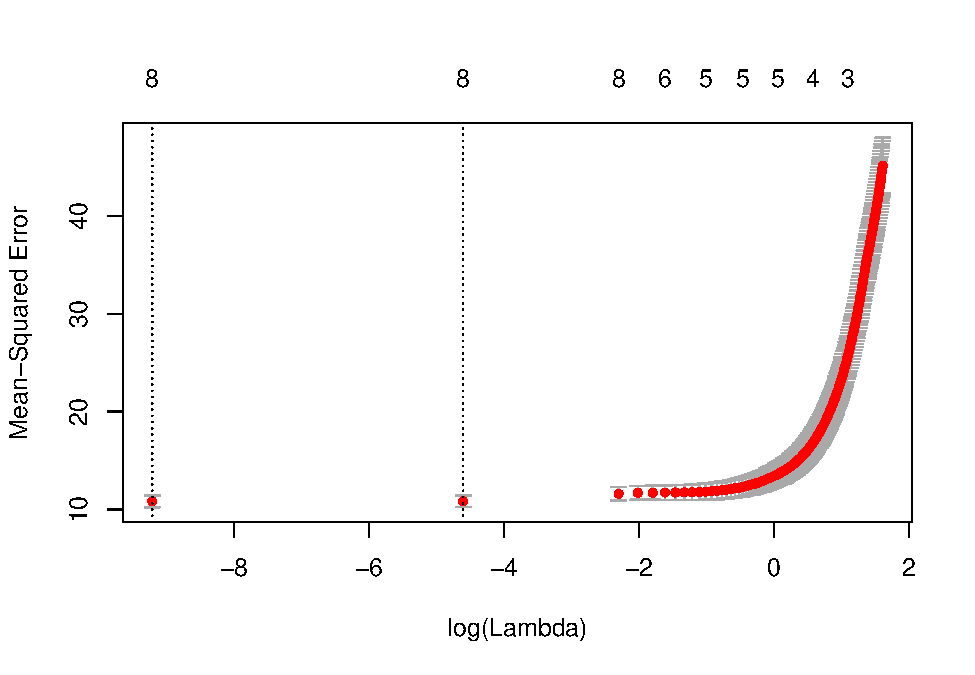
\includegraphics{1_files/figure-latex/unnamed-chunk-5-1.pdf}

\subsection{\texorpdfstring{2b) Finding the optimal
\(\lambda\)}{2b) Finding the optimal \textbackslash{}lambda}}\label{b-finding-the-optimal-lambda}

\begin{itemize}
\tightlist
\item
  Q14: Explain what the function \texttt{cv.glmnet} does.
\item
  Q15. Explain what we see in the above plot.
\item
  Q16: Finding the optimal lambda:
\end{itemize}

\begin{Shaded}
\begin{Highlighting}[]
\CommentTok{# need some R code here}
\end{Highlighting}
\end{Shaded}

\subsection{3c) Prediction}\label{c-prediction}

\begin{itemize}
\tightlist
\item
  Q17: Fit model, coefficients,\ldots{}
\end{itemize}

\begin{Shaded}
\begin{Highlighting}[]
\CommentTok{# fit the lasso}
\end{Highlighting}
\end{Shaded}

\begin{Shaded}
\begin{Highlighting}[]
\CommentTok{# 0 for cylinder, displace, horsepower, weight, acceleration, year, 0 for origin2 and 0 for origin3}
\NormalTok{newx=}\KeywordTok{matrix}\NormalTok{(}\KeywordTok{c}\NormalTok{(}\DecValTok{0}\NormalTok{,}\DecValTok{150}\NormalTok{,}\DecValTok{100}\NormalTok{,}\DecValTok{3000}\NormalTok{,}\DecValTok{10}\NormalTok{,}\DecValTok{82}\NormalTok{,}\DecValTok{0}\NormalTok{,}\DecValTok{0}\NormalTok{),}\DataTypeTok{nrow=}\DecValTok{1}\NormalTok{)}
\CommentTok{# then do the prediction}
\end{Highlighting}
\end{Shaded}

\begin{itemize}
\tightlist
\item
  Q18: Predicted value:
\end{itemize}

\subsection{3a)}\label{a-1}

\begin{itemize}
\tightlist
\item
  Q19: Fitting the specified \texttt{gam}
\end{itemize}

\begin{Shaded}
\begin{Highlighting}[]
\KeywordTok{library}\NormalTok{(gam)}
\CommentTok{# write R code}
\end{Highlighting}
\end{Shaded}

\begin{itemize}
\tightlist
\item
  Q20: The cubic spline basis.
\end{itemize}


\end{document}
